% Section 3.9: User Interface Design Principles

\section{3.9 User Interface Design Principles}
\label{sec:ui-design}
\addcontentsline{toc}{section}{3.9 User Interface Design Principles}

\lettrine{T}{his section} explores Symphony's user interface design philosophy and the interaction paradigms that enable effective human-AI collaboration. We examine the visual workflow composition system, real-time feedback mechanisms, and accessibility features that make Symphony both powerful and approachable. The interface design emphasizes clarity of intent, progressive disclosure, and multi-modal interaction to support diverse development scenarios and user preferences.

\subsection*{3.9.1 AI-First Interaction Paradigm and Visual Composition}
\addcontentsline{toc}{subsection}{3.9.1 AI-First Interaction Paradigm and Visual Composition}

\lettrine{T}{he} user interface design of Symphony embodies a fundamental rethinking of how developers interact with AI-powered development environments. The design philosophy recognizes that traditional code-centric interfaces are insufficient for environments where AI agents handle much of the implementation work, and that new interaction paradigms are needed to enable effective human-AI collaboration. The interface design emphasizes clarity of intent over precision of instruction, visual representation of complex workflows over textual descriptions, and real-time feedback about AI activities over passive waiting for results.

The AI-first interaction paradigm shifts the developer's role from writing detailed instructions to providing high-level guidance and making strategic decisions. The interface supports this paradigm shift by providing mechanisms for expressing intent through natural language prompts, visualizing how the system interprets and plans to execute those intents, enabling developers to review and refine automatically generated plans before execution, and providing comprehensive visibility into AI activities during execution. This interaction model reduces cognitive load by eliminating the need to specify every detail while maintaining developer control through review and approval mechanisms.

The visual workflow composition capabilities provided by the Harmony Board enable developers to create and understand complex workflows through direct manipulation rather than textual programming. The interface presents workflows as node-and-edge graphs where nodes represent individual tasks and edges represent data dependencies. Developers can drag nodes from a palette onto the canvas to add tasks, draw edges between nodes to establish dependencies, configure node parameters through property panels, and arrange the layout to improve clarity. This visual approach makes workflow structure immediately apparent and enables developers to reason about complex processes more effectively than textual representations would allow.

The Harmony Board creation process involves multiple steps that guide developers from initial concept to executable workflow. The process begins with opening the Harmony Board in creation mode and loading the palette of available extensions. Developers drag nodes representing Instruments, Operators, and Motifs onto the canvas to build the workflow structure. The system validates connections in real-time as developers draw edges between nodes, providing immediate feedback about type compatibility and other constraints. Developers configure parameters for each node, specifying inputs, resource limits, and other settings. The system validates the complete workflow to ensure it forms a valid directed acyclic graph with no cycles or type mismatches. Once validation passes, developers can save the workflow to the Polyphony Store and optionally publish it for others to use. As illustrated in Figure 3.14, this complete creation process demonstrates the visual workflow composition capabilities.

\begin{figure}[H]
\centering
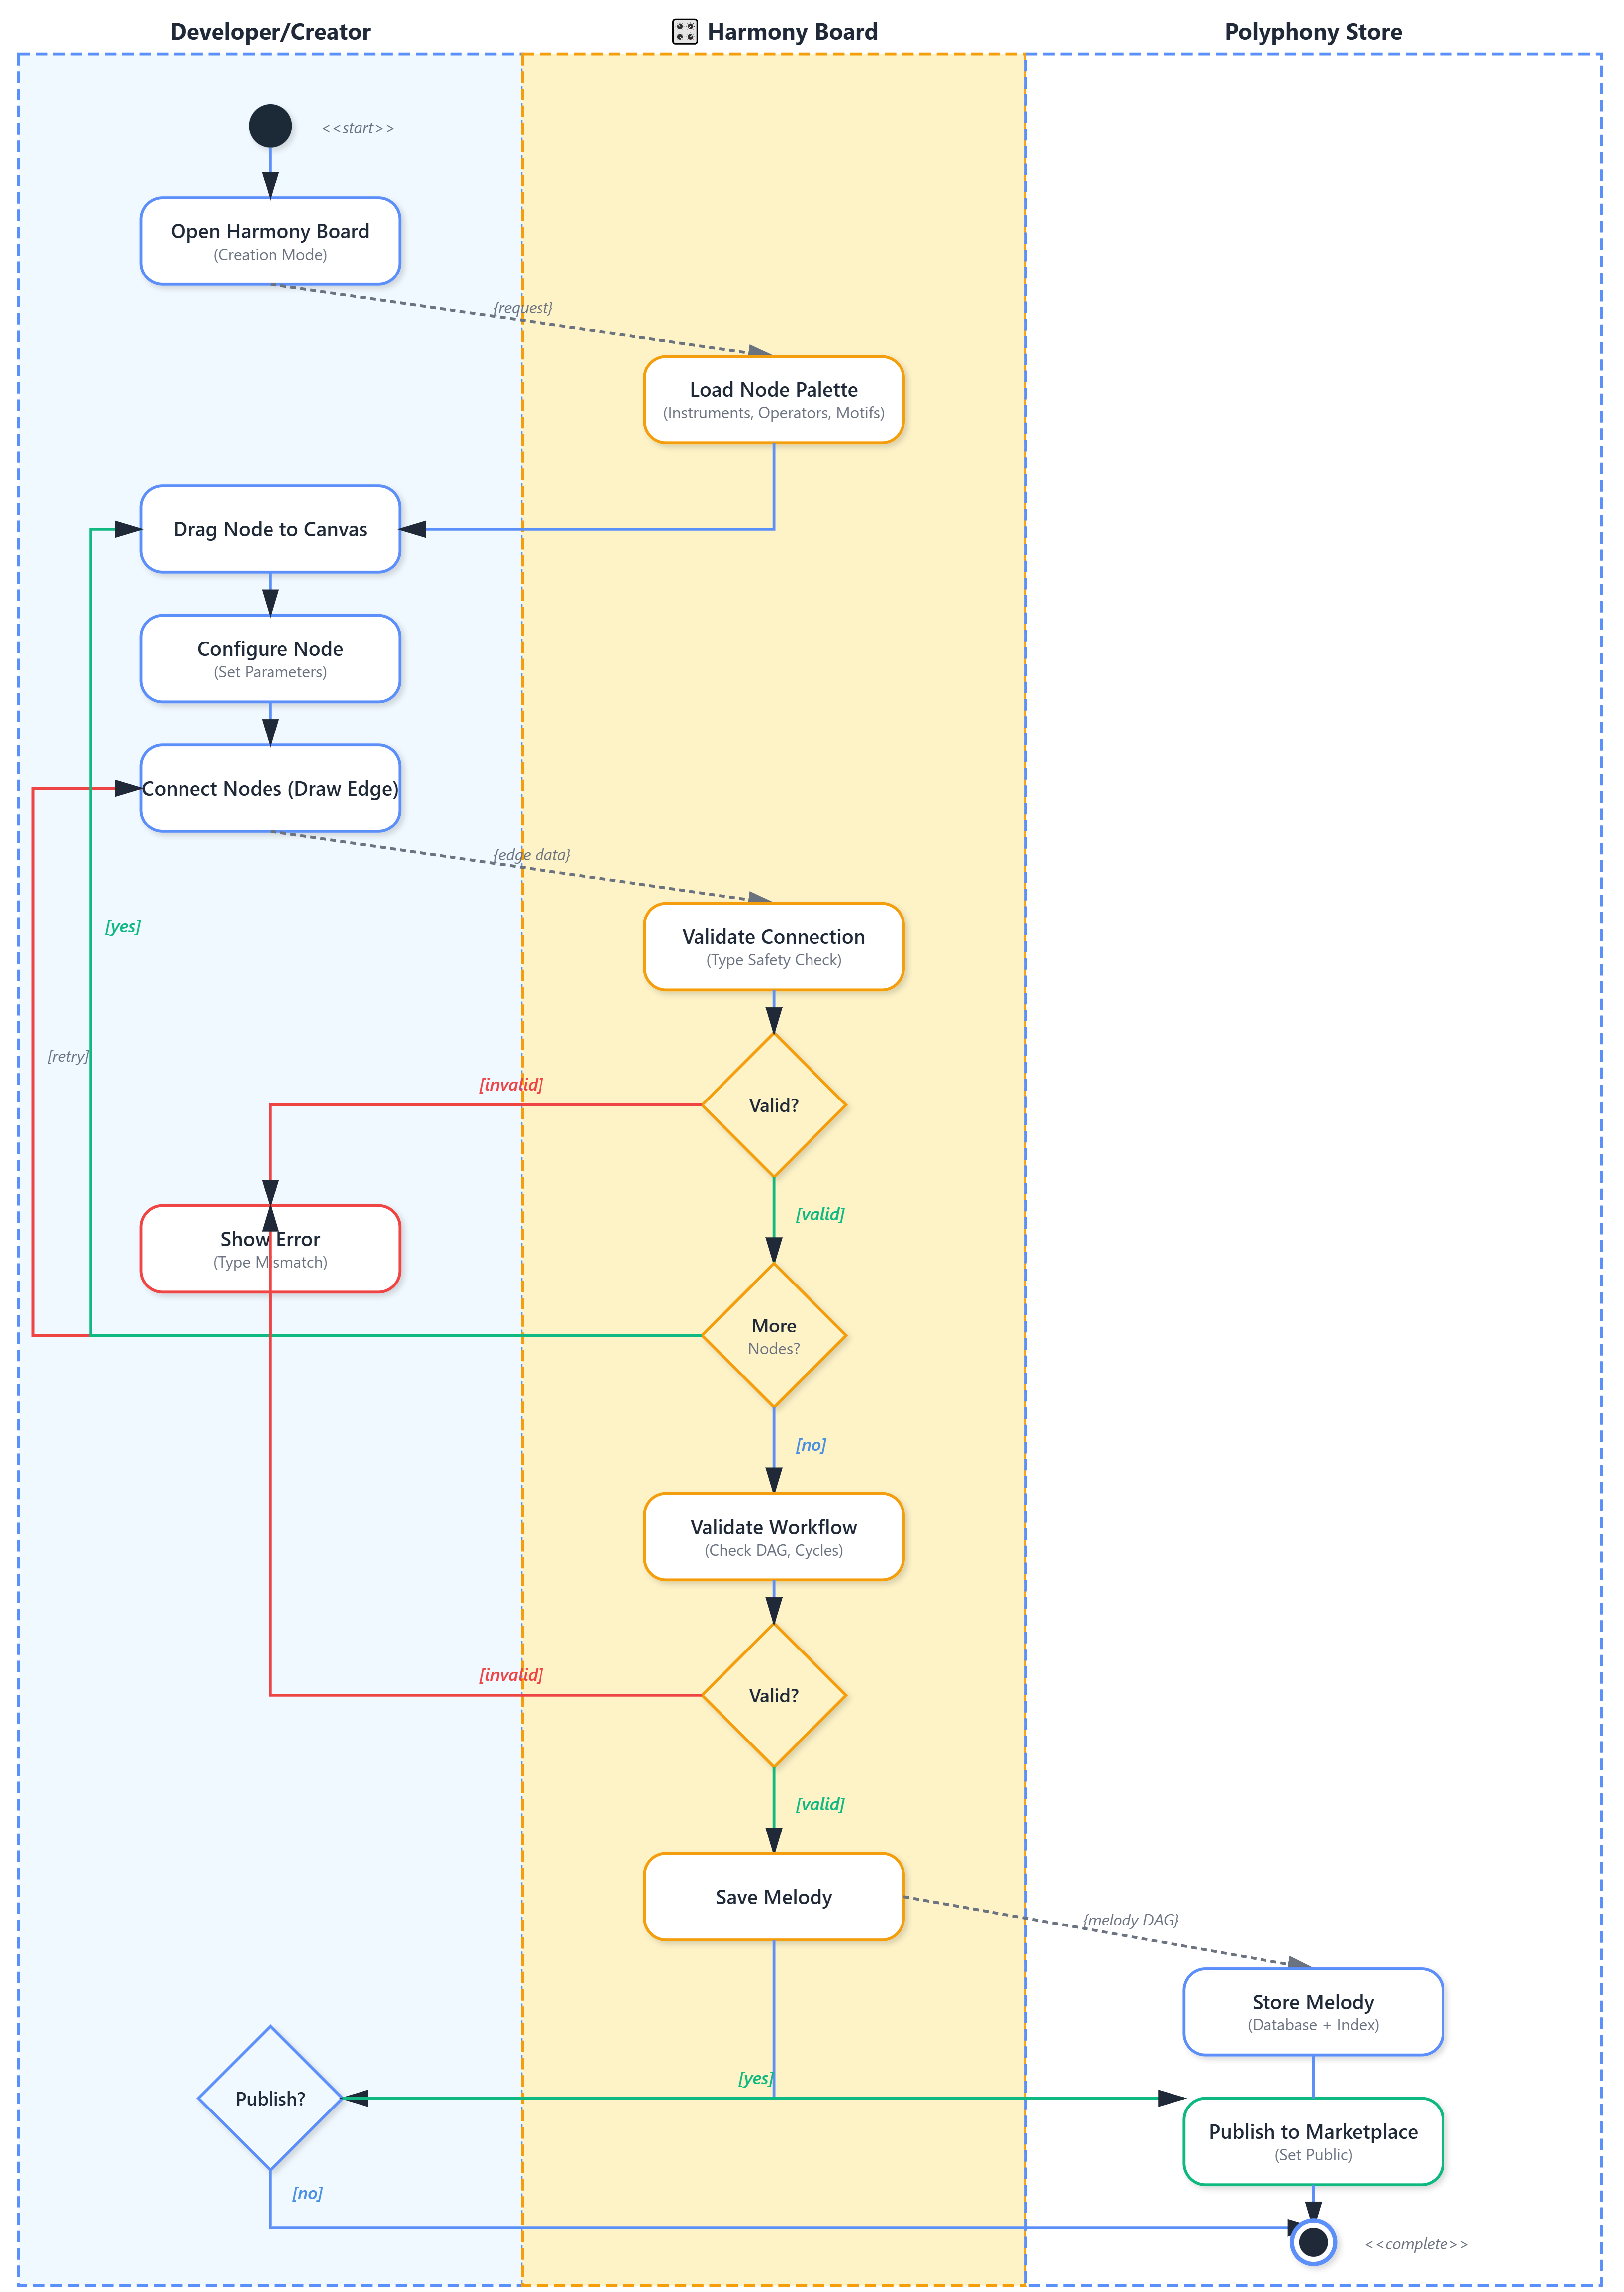
\includegraphics[width=0.95\textwidth]{images/diagrams/activity_diagram/symphony-harmony-board-creation.png}
\caption{Harmony Board Creation Process}
\label{fig:3.14-harmony-board-creation}
\end{figure}

\subsection*{3.9.2 Feedback, Context Awareness, and User Experience}
\addcontentsline{toc}{subsection}{3.9.2 Feedback, Context Awareness, and User Experience}

The real-time feedback mechanisms keep developers informed about AI activities through progress indicators showing task execution status, completion percentage, and estimated time remaining. The interface highlights errors immediately with stack traces and diagnostic information, building trust through transparency. Context-aware assistance adapts based on current development context, suggesting relevant workflows and highlighting applicable extensions to reduce cognitive burden.

The progressive disclosure approach manages complexity by showing essential information by default while making advanced details available on demand. Multi-modal interaction enables developers to use natural language prompts, visual workflow composition, direct code editing, or voice commands based on task requirements and preferences. Collaborative features support real-time multi-developer workflows with change tracking, attribution, and workflow sharing through the Polyphony Store.

Accessibility considerations ensure broad usability through keyboard navigation, screen reader compatibility, customizable color schemes including high-contrast modes, and adjustable font sizes for diverse developer abilities and preferences.

\subsection*{3.9.3 System Integration and User Empowerment}
\addcontentsline{toc}{subsection}{3.9.3 System Integration and User Empowerment}

Performance optimization ensures responsive interface through virtual scrolling, lazy loading, incremental rendering, and background processing. Error presentation shows issues in context with suggested fixes and quick actions for retry or rollback. Workspace management enables independent configuration of multiple environments with different extensions, settings, and workflows for different projects or contexts.

Customization capabilities support custom color themes, keyboard shortcuts, layouts, and extensions to match individual preferences. Integration with external tools displays information from issue trackers, version control, and CI services, enabling Symphony to complement existing development infrastructure. Performance monitoring provides execution time, resource utilization, bottleneck identification, and historical trends for workflow optimization.

The design principles emphasize clarity through understandable system behavior, efficiency through minimized steps for common tasks, and empowerment by giving developers control over AI activities while reducing routine task burden. These principles ensure that Symphony's interface serves developers effectively while supporting the AI-first development paradigm. As shown in Figure 3.15, the diverse use cases demonstrate the system's flexibility and breadth of functionality.

\begin{figure}[H]
\centering
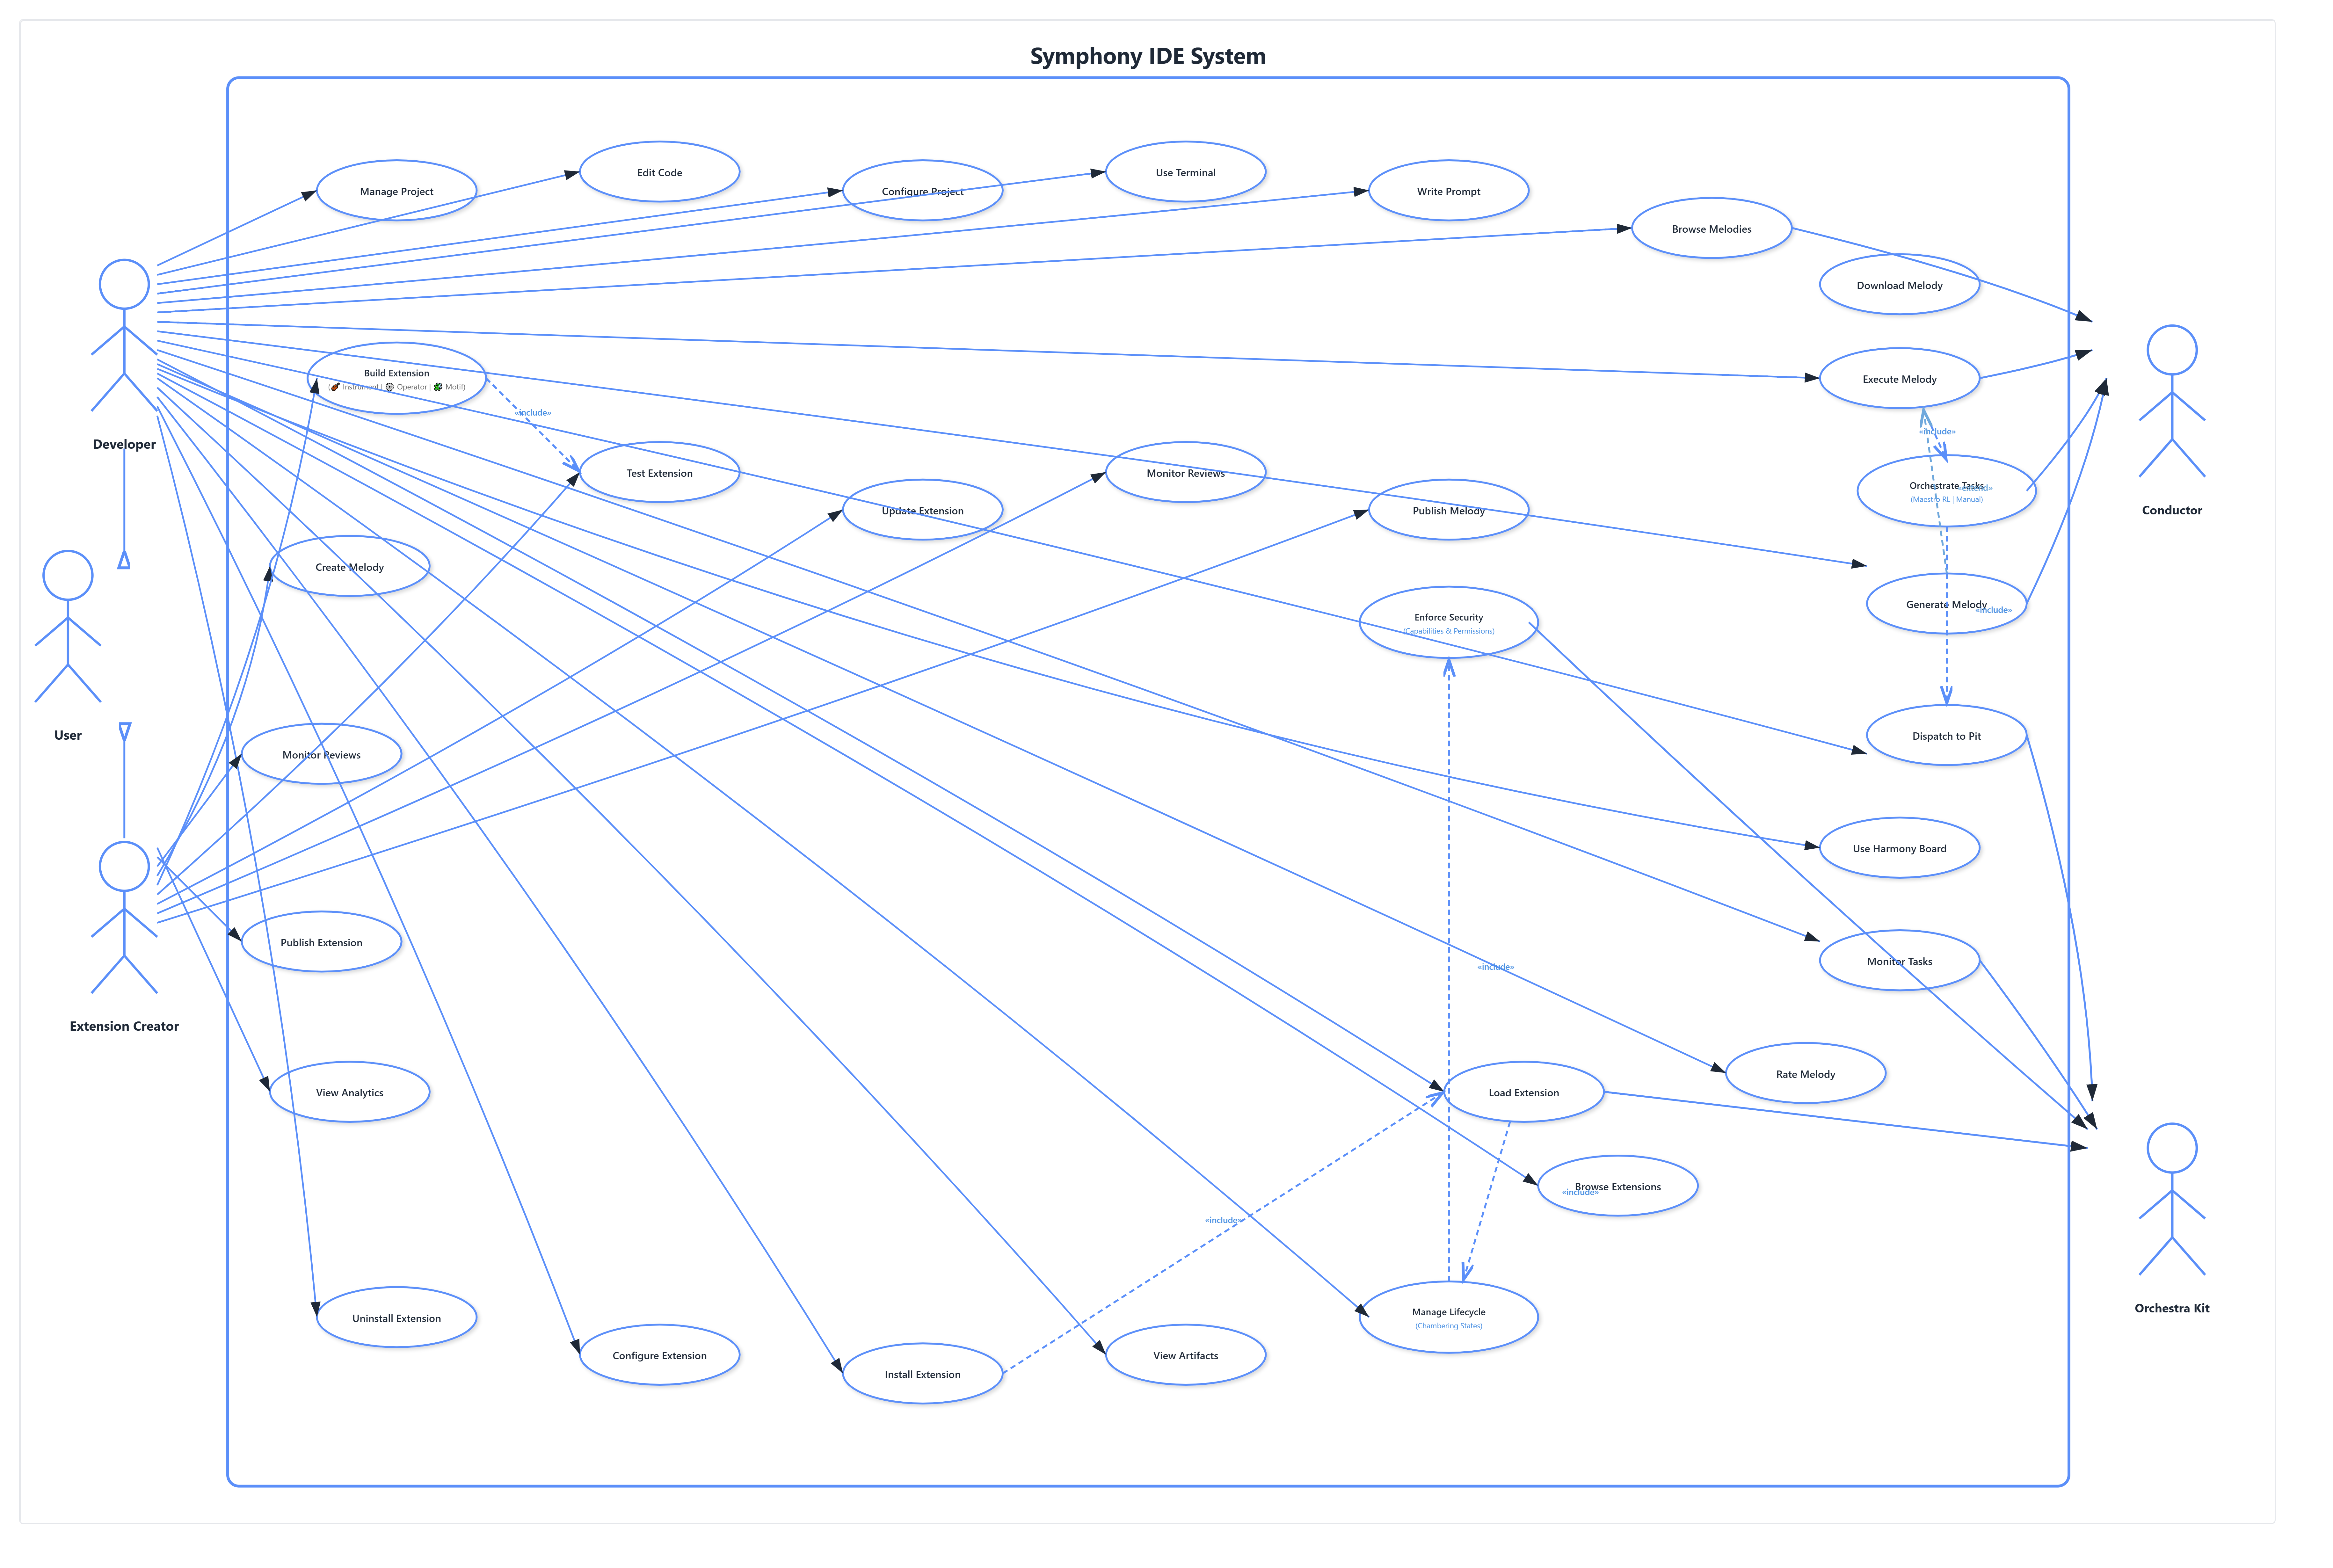
\includegraphics[width=0.85\textwidth]{images/diagrams/use-case.png}
\caption{System Use Cases}
\label{fig:3.15-use-cases}
\end{figure}
